\chapter{Modelling the ROV} \label{cha:modelling}
This chapter describes how the \abbrROV is modelled using the \citet{fossen2011} 6 \abbrDOF model for \abbrROV:s. A model describes how an object is affected by forces such as gravity and friction. Models are derived by using different physical laws. Assumptions can often be made how the physical properties of the object affect the model and a simpler model can be derived. Assumptions can be symmetry of the object, no coupling inertia, low speed and several others. 

An underwater vehicle with 6 \abbrDOF can be described by\index{Model of an underwater vehicle}
\begin{equation}
\etaVectordot = J(\eta)\nu
\end{equation}

\begin{equation} \label{eq:model}
 \inertia \nuVectordot + \coriolis(\nuVector)\nuVector + \damping(\nuVector)\nuVector + \gravity(\etaVector) = \tauVector
\end{equation}
 
where
\begin{equation*}
  \etaVector  
\end{equation*} are generalised positions and
\begin{equation*}
  \nuVector
\end{equation*}
are generalised velocities that are used to describe motion in 6 \abbrDOF \citep[p. 15]{fossen2011}. The matrices $\inertia$\index{Inertia matrix}, $\coriolis(\nuVector)$\index{Coriolis matrix}, $\damping(\nuVector)$\index{Damping matrix} and the vector $\gravity(\nuVector)$\index{Restoring forces matrix} respectively describes how inertia, Coriolis forces, damping forces, gravity and buoyancy affect the \abbrROV. The vector $\tauVector$ describes the forces and torques produced by the \abbrROV's actuators as well as environmental disturbances.
 
%%%%%%%%%%%%%%%%%%%%%%%%%%%%%%%%%%%%%%%%
In this chapter, the vector cross-product $\cross{\cdot}$ is defined as $\cross{a\boldsymbol{A}} \boldsymbol{B} = a\boldsymbol{A} \times \boldsymbol{B}$. The notation used for the parameters in this chapter and \Chapterref{cha:parameterEstimation} can be seen in \Tableref{tab:notationModelling}. The notation for forces, moments, linear and angular velocities, positions and Euler angles used in the model is summarised in \Tableref{tab:notationMarine}. 

 \begin{table}[tbp]
  \centering
  \caption{\label{tab:notationModelling}%
    The notation and description of the parameters used in the \abbrROV model.}

  \begin{tabular}{l p{0.7\linewidth}}
    \toprule%
    \textbf{Notation} & \textbf{Description} \\
    \otoprule%
    $\bodyinertia{b}$ & Inertia matrix for rotation around \abbrCO.\\
    $\bodyinertia{g}$ & Inertia matrix for rotation around \abbrCG.\\
    $\Kp, \Mq,\Nr$    & Linear damping coefficients for rotation in water. \\
    $\Kpabsp, \Mqabsq,\Nrabsr$ & Quadratic damping coefficients for rotation in water. \\
    $\Kpdot, \Mqdot,\Nrdot$    & Increased inertia about $\xPosition, \yPosition, \zPosition$-axis due to rotation in water.\\
    $\Xu, \Yv, \Zw$ & Linear damping coefficients for translation in water.\\
    $\Xuabsu, \Yvabsv, \Zwabsw$ & Quadratic damping coefficients for translation in water.\\
    $\Xudot, \Yvdot, \Zwdot$   & Added mass in $\xPosition, \yPosition, \zPosition$-direction due to translation in water. \\
    $\distance{x}{i}, \distance{y}{i},\distance{z}{i}$. & Moment arms from \abbrCG to each thruster $i$. \\
    $m$ & The \abbrROV's mass \\
    $z_B$ & Distance between \abbrCB and \abbrCG along the $z$-axis. \\
    $V$ & Displaced volume. \\
    $\rho$ & Water density. \\
    $g$ & Gravity. \\
    $r^g_b$ & The distance between \abbrCO and \abbrCG. \\
    \bottomrule%
  \end{tabular}
\end{table}

 \begin{table}[tbp]
  \centering
  \caption{\label{tab:notationMarine}%
    The notation of \citet{sname} for marine vessels.}

  \begin{tabular}{l p{0.35\linewidth}  p{0.14\linewidth} p{0.14\linewidth} p{0.14\linewidth}}
    \toprule%
    \textbf{DOF} & \textbf{Description}  & \textbf{Forces and moments} & \textbf{Linear and angular velocities} & \textbf{Positions and Euler angles} \\
    \otoprule%
    1 & Motions in the x direction (surge).     & \xForce       & \xVelocity        & \xPosition \\
        
    2 & Motions in the y direction (sway).      & \yForce       & \yVelocity        & \yPosition \\
    
    3 & Motions in the z direction (heave).     & \zForce       & \zVelocity        & \zPosition \\
    
    4 & Rotation about the x axis (roll, heel). & \rollMoment   & \rollVelocity     & \rollAngle \\
    
    5 & Rotation about the y axis (pitch, trim).& \pitchMoment  & \pitchVelocity    & \pitchAngle \\
    
    6 & Rotation about the z axis (yaw).        & \yawMoment    & \yawVelocity      & \yawAngle \\
    \bottomrule%
  \end{tabular}
\end{table}

To get a more compact way of writing a vector notation has been used
\begin{itemize}
\item $\boldsymbol{p}$: Positions.
\item $\boldsymbol{v}$: Linear velocities.
\item $\boldsymbol{\eulerAngles}$: Euler Angles.
\item $\boldsymbol{\quaternion}$: Quaternions.
\item $\boldsymbol{\omega}$: Angular velocities.
\end{itemize}

%%%%%%%%%%%%%%%%%%%%%%%%%%%%%%%%%%%%%%%%
\section{Coordinate Systems and Kinematics}
\label{sec:coordinates}\index{NED}\index{body-fixed coordinate system}\index{global coordinate system}
During modelling it is important to choose proper coordinate systems in which to describe the systems behaviour.
In this thesis, are two coordinate systems used in the \abbrROV model.
The first system, the body-fixed coordinate system, is fixed to the \abbrROV and rotates with the \abbrROV. 
The body-fix coordinate system is a right-hand system, the $\xPosition$-axis is placed along the length of the \abbrROV pointing towards its bow. The $\yPosition$-axis points starboard, and the $\zPosition$-axis points downwards towards the vehicles keel. The coordinate system is assumed to be centred in the \abbrROV's  center of gravity (\abbrCG). The body-fixed coordinate system makes it easier to describe sensor readings, since the sensors rotate with the \abbrROV. It is also easier to express the effect of each thruster with forces and moments expressed in the body-fixed coordinate system. How the body-fixed coordinate system is placed in the \abbrROV can be seen in \Figureref{fig:thrusterlocationtop} and \Figureref{fig:thrusterlocationfront}.

The global coordinate system is Earth fixed, with axes $\north$, $\east$ and $\down$. The $\north$ axis points in the direction of the calibrated North, the $\east$ axis points in the direction of calibrated East and the $\down$ axis points down towards the \abbrCG of the Earth.
This coordinate system is used to express buoyancy and gravitational forces acting on the \abbrROV, their effects are transformed to the body-fixed coordinate system by a rotation matrix. How the local and global coordinate systems relate to each other can be seen in \Figureref{fig:coordinate_frames}.

\newcommand*{\coordinateRadius}{0.05}
\newcommand*{\coordRot}{30}
\begin{figure}
\centering 
\begin{tikzpicture}
    \node[anchor=south west,inner sep=0] (image) at (0,0) {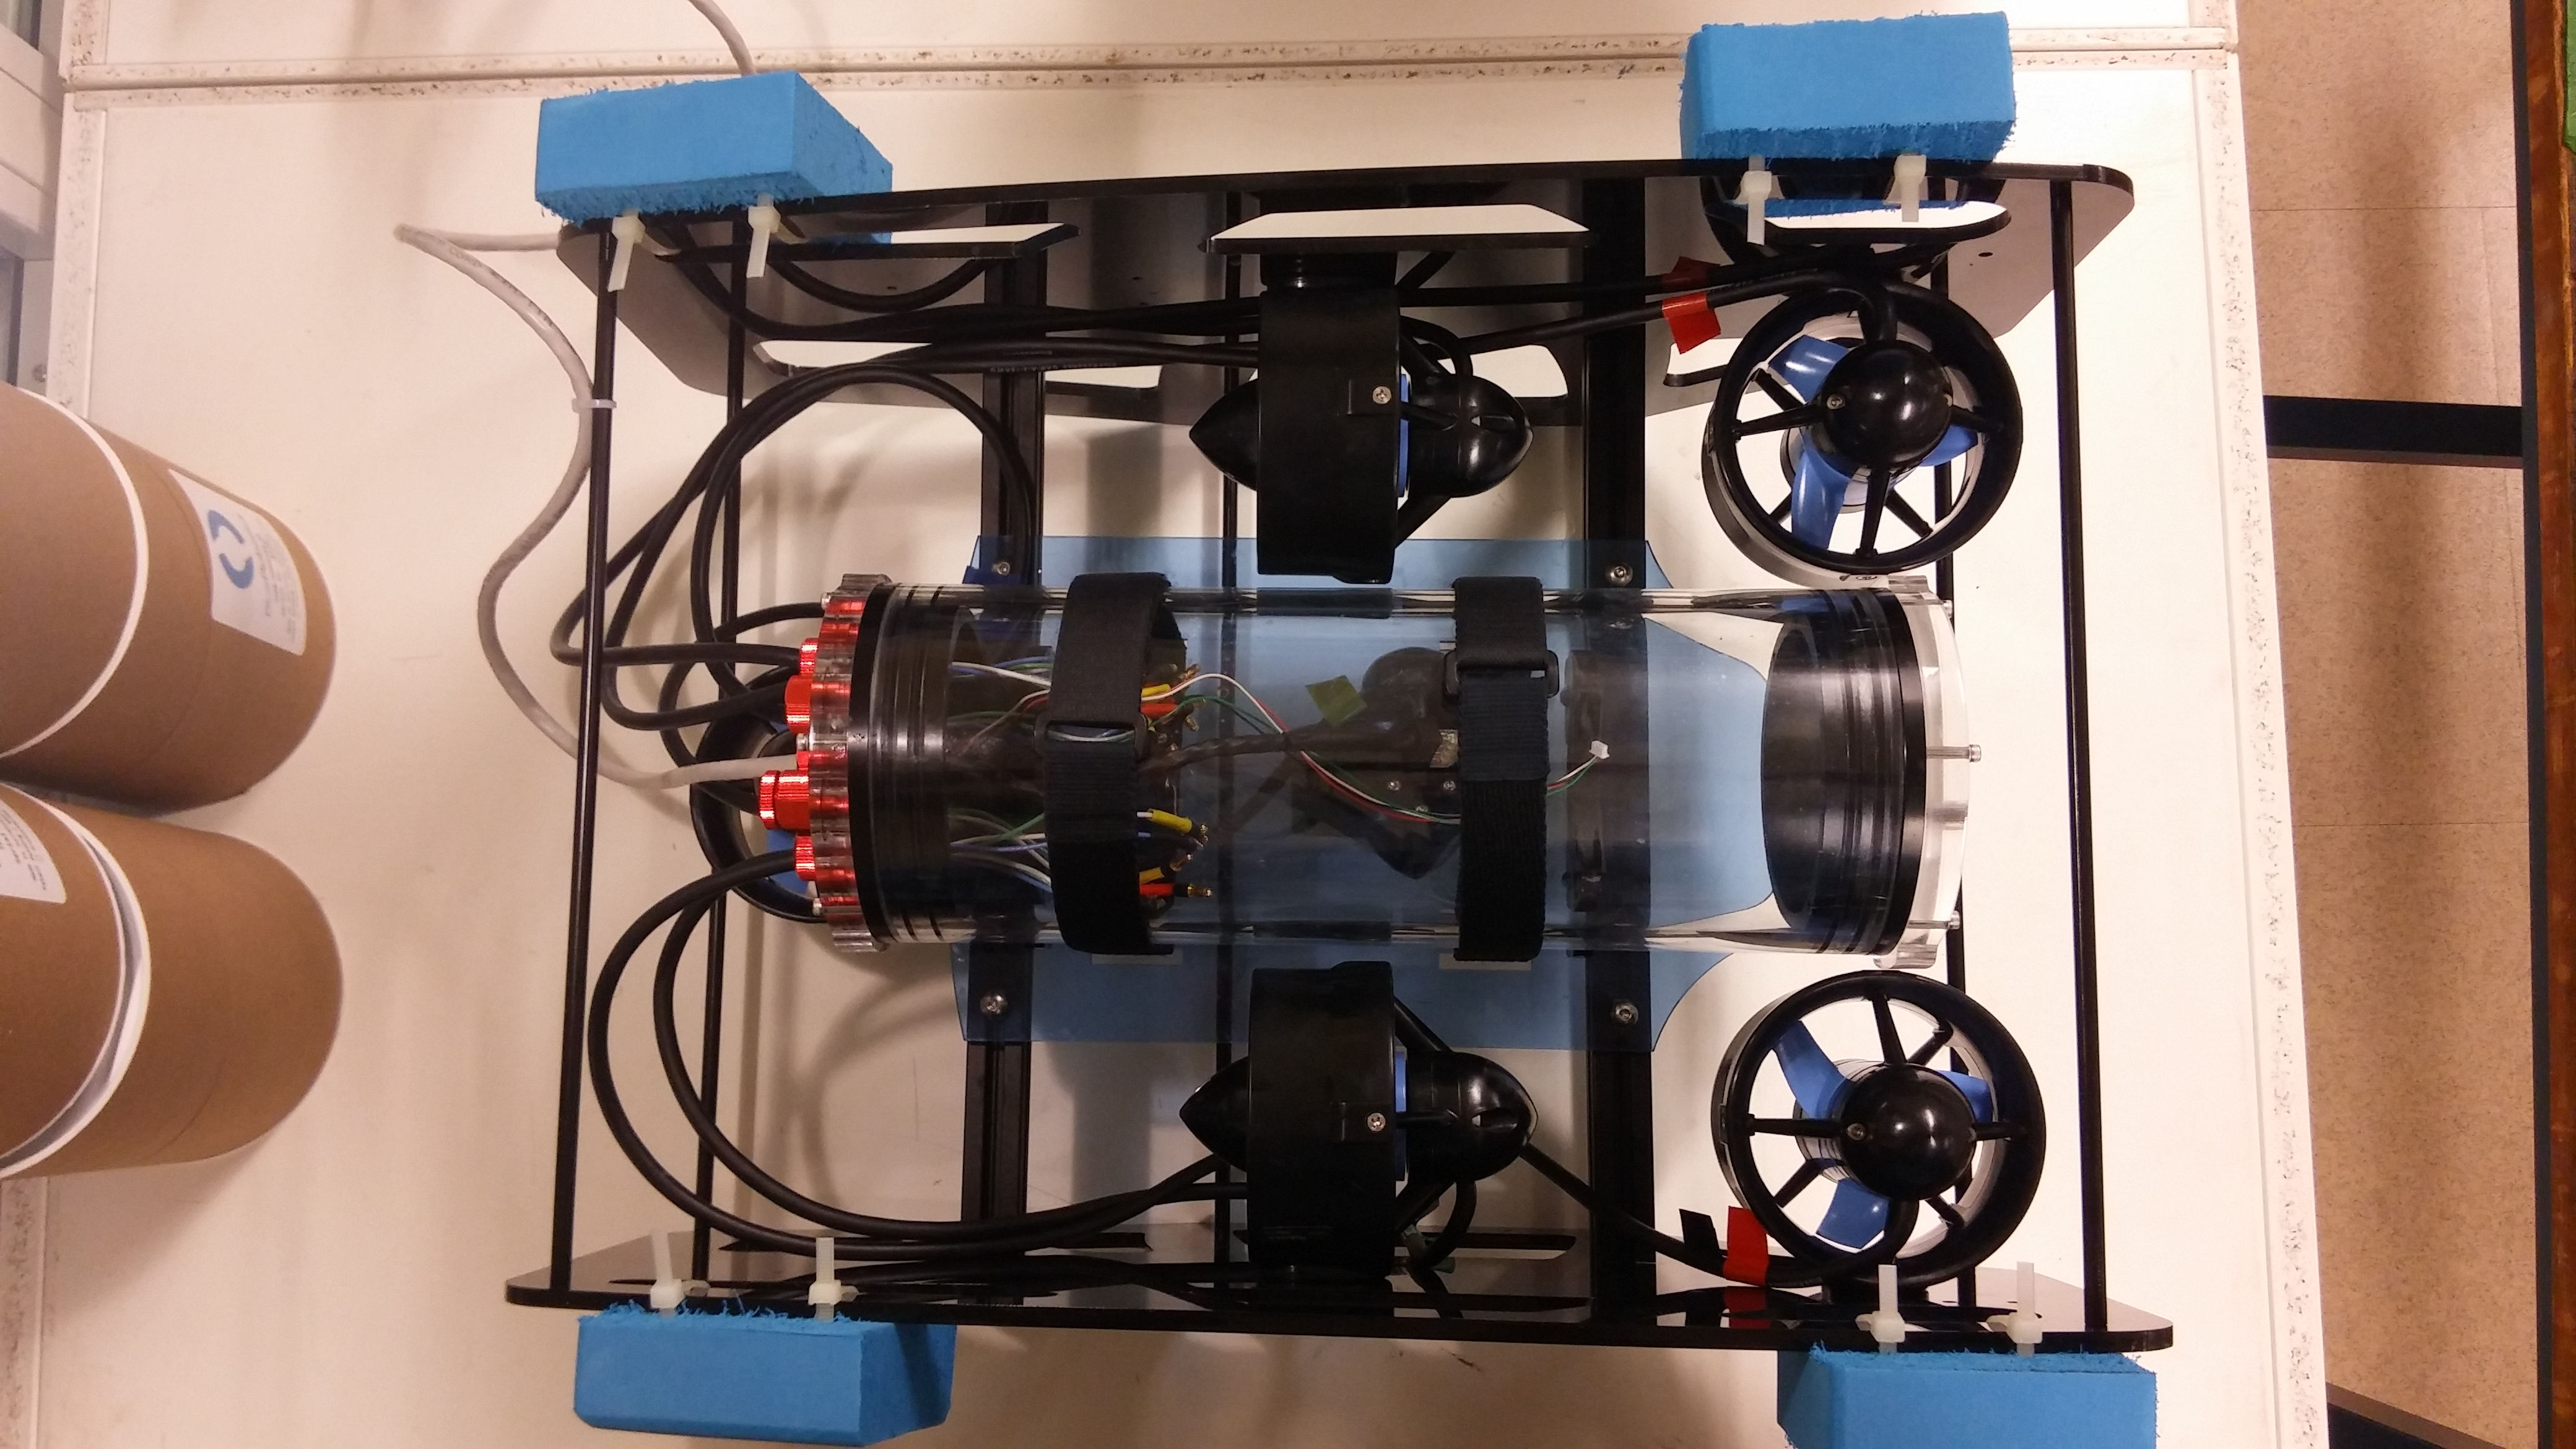
\includegraphics[trim={28cm 0cm 22cm 5cm},clip,width=0.9\textwidth]{thrusterlocationtop}};
    \begin{scope}[x={(image.south east)},y={(image.north west)}]
		\pgfmathsetmacro\coordinateRadius{0.025}
        \pgfmathsetmacro\by{\coordinateRadius*sin(45)}
        \pgfmathsetmacro\bx{\coordinateRadius*cos(45)}
        \pgfmathsetmacro\ay{\coordinateRadius*sin(\coordRot)}
        \pgfmathsetmacro\ax{\coordinateRadius*cos(\coordRot)}
        \pgfmathsetmacro\coordYRot{sin(\coordRot)}
        \pgfmathsetmacro\coordXRot{cos(\coordRot)}
        
        \coordinate (O) at (0.48,0.52);
        \draw[red, ultra thick,->] (O) ++(\coordinateRadius,0) -- ++(0.4,0) node[anchor=north east]{\large\color{red}$\xPosition$};
        \draw[red, ultra thick,->] (O) ++(0,-\coordinateRadius)-- ++(0,-0.4) node[anchor=south east]{\large\color{red}$\yPosition$};
        \draw[red, ultra thick] (O) circle (\coordinateRadius); 
        \draw[red, ultra thick] (O) ++(0,\coordinateRadius) node[above]{\large\color{red}$\zPosition$};
        \draw[red, ultra thick] (O) -- ++(\bx,\by) (O) -- ++(-\bx,-\by) (O) -- ++(-\bx,\by) (O)  -- ++(\bx,-\by);
        
        \draw[yellow, ultra thick, <->] (O) ++(0.34,0) -- ++(0,0.23)  node [midway, left] {\large\distance{y}{1}};
        \draw[red, ultra thick] (O) ++(0.34,0.23) node[right]{\large Thruster 1};
        \draw[yellow, ultra thick, <->] (O) ++(0.34,0) -- ++(0,-0.28) node [midway, left] {\large\distance{y}{2}};
        \draw[red, ultra thick] (O) ++(0.34,-0.28) node[right]{\large Thruster 2};
        \draw[yellow, ultra thick, <->] (O) ++(0.03,0) -- ++(0,0.24)  node [midway, right] {\large\distance{y}{3}};
        \draw[red, ultra thick] (O) ++(0.03,0.24) node[right]{\large Thruster 3};
        \draw[yellow, ultra thick, <->] (O) ++(0.03,0) -- ++(0,-0.28) node [midway, right] {\large\distance{y}{4}};
        \draw[red, ultra thick] (O) ++(0.03,-0.28) node[right]{\large Thruster 4};
        
        \draw[yellow, ultra thick, <->] (O) ++(0,0.27) -- ++(0.34,0)  node [midway, above] {\large\distance{x}{1}};
        \draw[yellow, ultra thick, <->] (O) ++(0,-0.32) -- ++(0.34,0)  node [midway, below] {\large\distance{x}{2}};
        \draw[yellow, ultra thick, <->] (O) -- ++(-0.30,0)  node [midway, below] {\large\distance{x}{5}};
        \draw[red, thick] (O) ++(-0.35,0) node[rotate=90]{\large Thruster 5};
    \end{scope}
\end{tikzpicture}
    \caption{Top view of the \abbrROV. The red coordinate system illustrates how the body-fixed coordinate system is fixed in the \abbrROV. Yellow lines shows the different moment arms to the thrusters. Each thruster is numbered in red.}
    \label{fig:thrusterlocationtop}
\end{figure}

\begin{figure}
\centering 
\begin{tikzpicture}
    \node[anchor=south west,inner sep=0] (image) at (0,0) {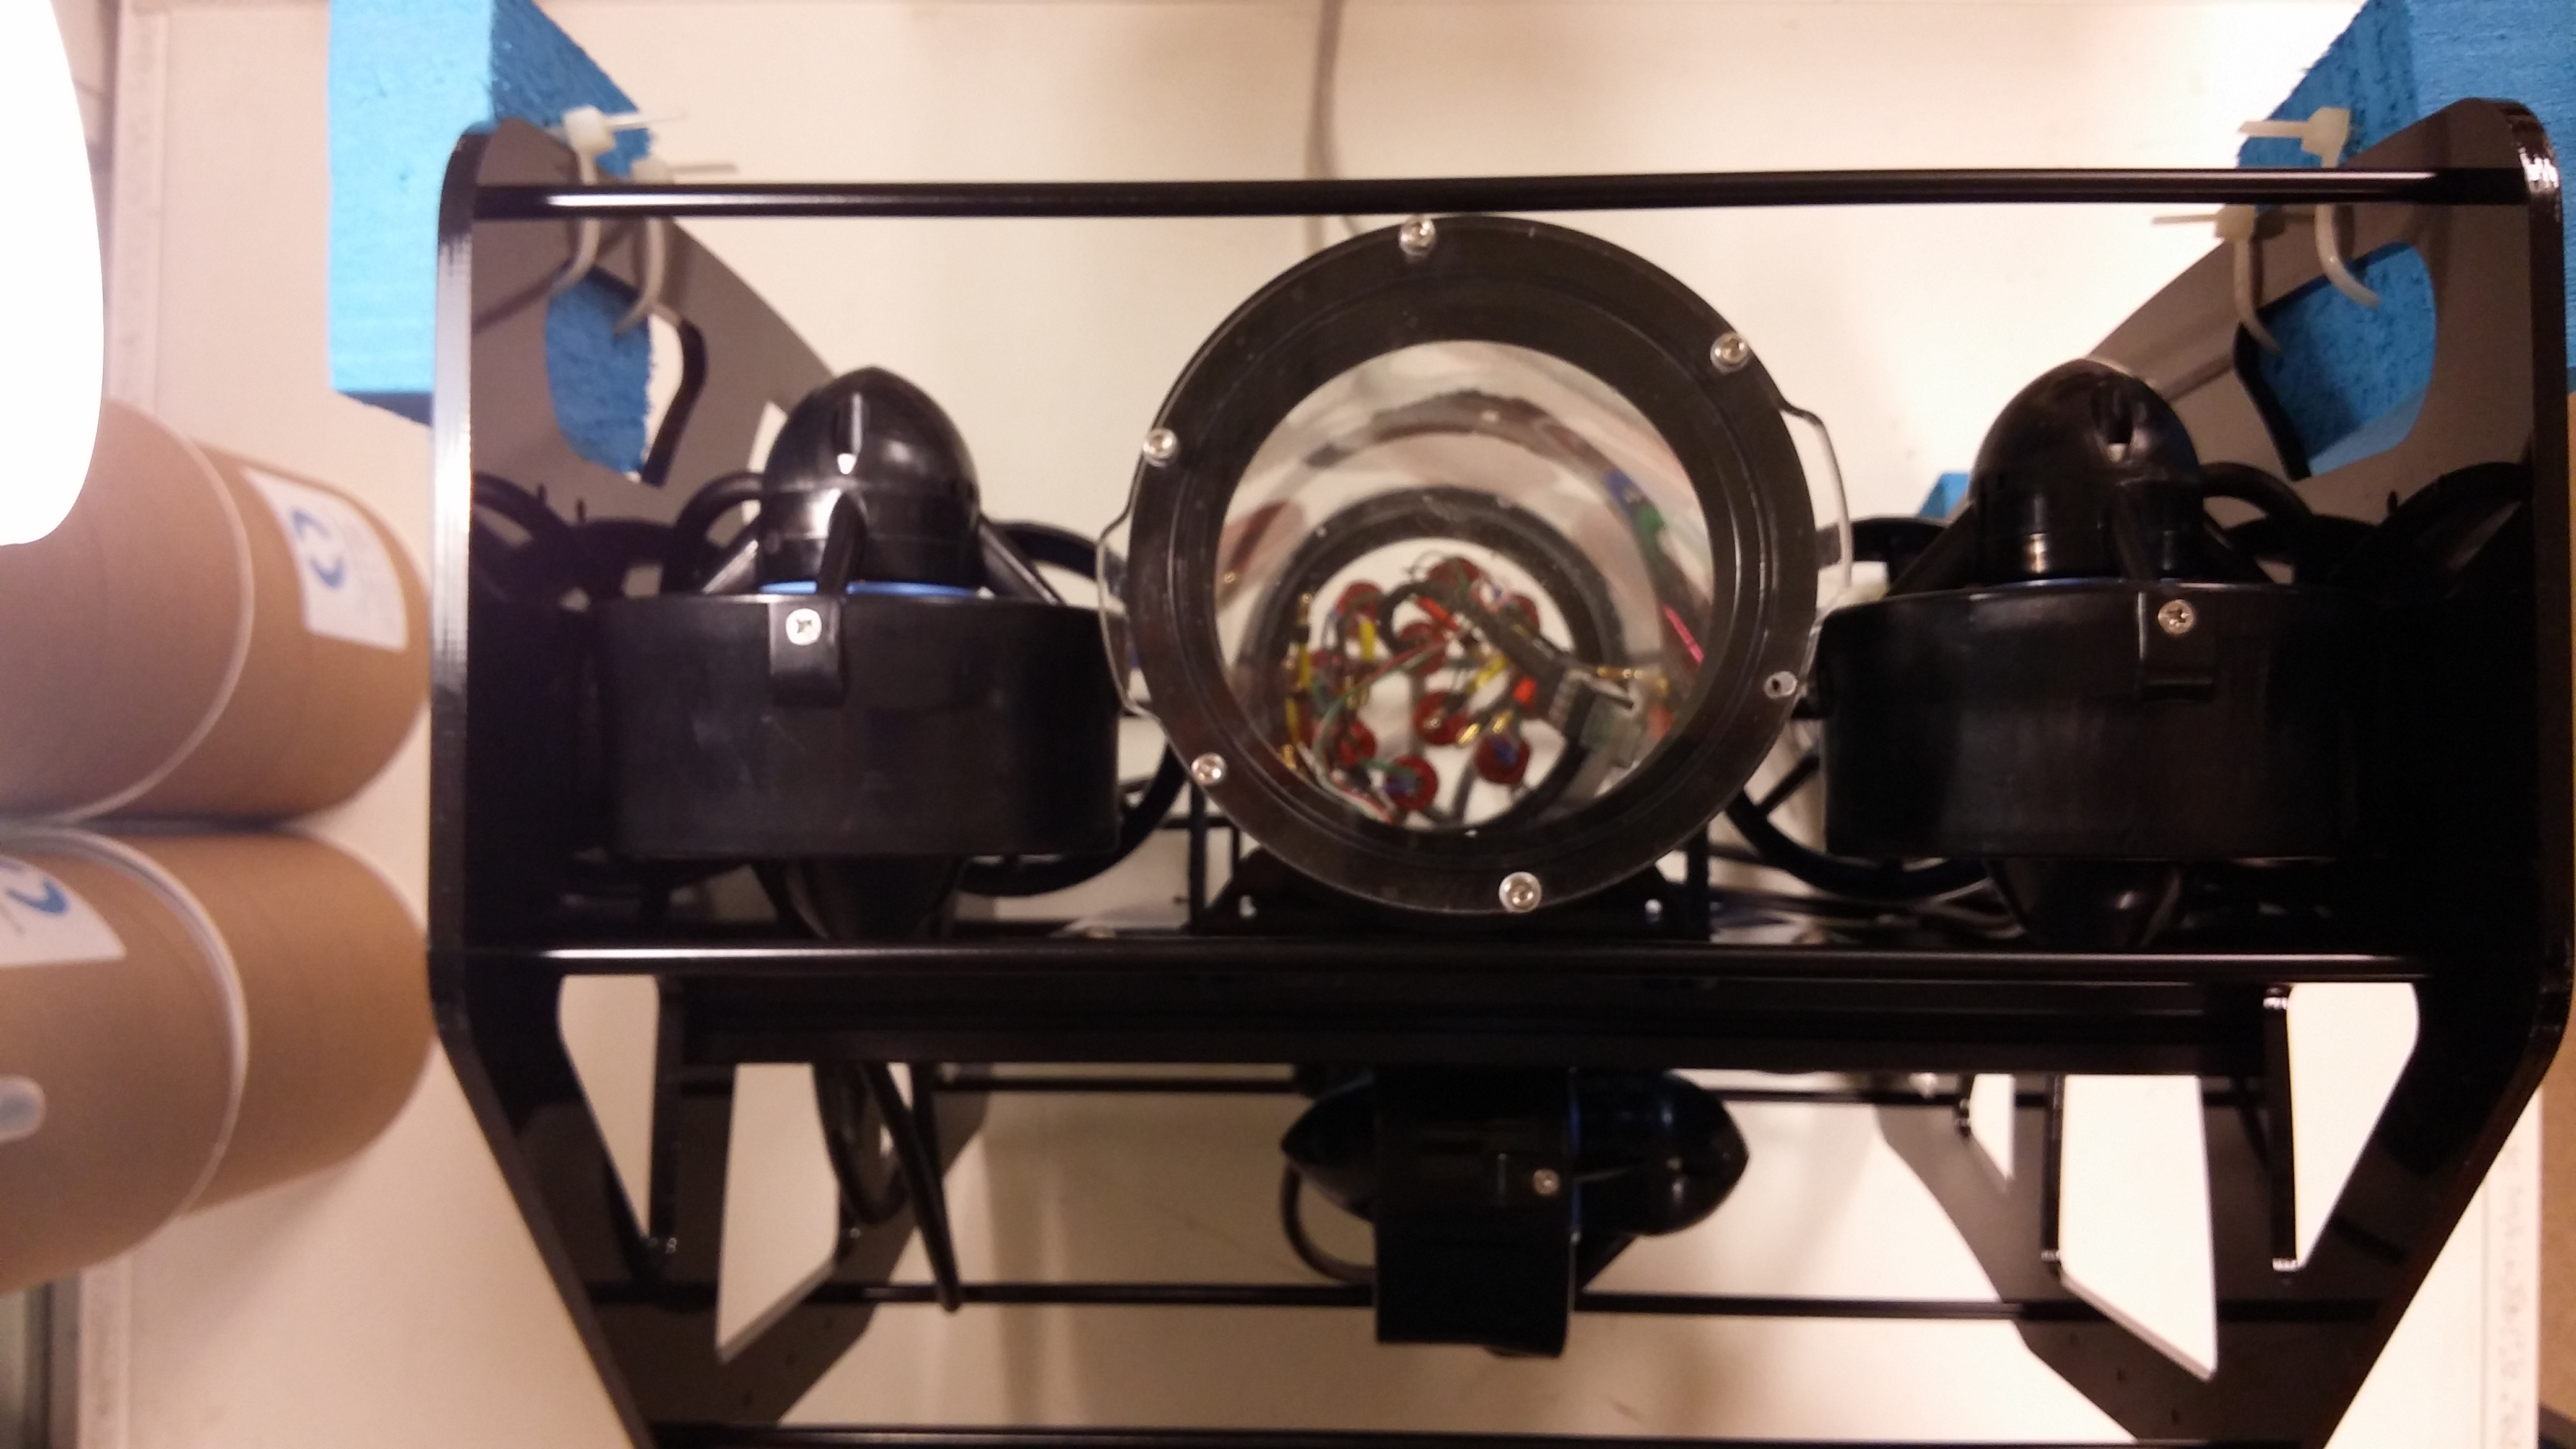
\includegraphics[trim={25cm 2cm 0cm 0cm},clip,width=0.9\textwidth]{thrusterlocationfront}};
    \begin{scope}[x={(image.south east)},y={(image.north west)}]
		\pgfmathsetmacro\coordinateRadius{0.025}
        \pgfmathsetmacro\by{\coordinateRadius*sin(45)}
        \pgfmathsetmacro\bx{\coordinateRadius*cos(45)}
        \pgfmathsetmacro\ay{\coordinateRadius*sin(\coordRot)}
        \pgfmathsetmacro\ax{\coordinateRadius*cos(\coordRot)}
        \pgfmathsetmacro\coordYRot{sin(\coordRot)}
        \pgfmathsetmacro\coordXRot{cos(\coordRot)}
        
        \coordinate (O) at (0.48,0.55);
        \draw[red, ultra thick,->] (O) ++(-\coordinateRadius,0) -- ++(-0.4,0) node[anchor=north east]{\large\color{red}$\yPosition$};
        \draw[red, ultra thick,->] (O) ++(0,-\coordinateRadius)-- ++(0,-0.5) node[anchor=south east]{\large\color{red}$\zPosition$};
        \draw[red, ultra thick] (O) circle (\coordinateRadius);        
        \draw[red, ultra thick] (O) ++(0,\coordinateRadius) node[above]{\large\color{red}$\xPosition$};
		\draw[red, ultra thick] (O) node[circle,fill,inner sep=1pt]{};
        
        \draw[yellow, thick, <->] (O) ++(0.04,0) -- ++(0,-0.37)  node [midway, right]{\large\distance{z}{6}};
        \draw[red, thick] (O) ++(0.04,-0.37) node[right]{\large Thruster 6};
    \end{scope}
\end{tikzpicture}
    \caption{Front view of the \abbrROV. The red coordinate system illustrates how the body-fixed coordinate system is fixed in the \abbrROV. The yellow line show the moment arm to thruster 6 which is marked in red.}
    \label{fig:thrusterlocationfront}
\end{figure}
\todo{update this figure with N' to indicate that the rotation is around the new axis}
\begin{figure}
    \centering
    \begin{tikzpicture}[scale=2]
        \pgfmathsetmacro\by{\coordinateRadius*sin(45)}
        \pgfmathsetmacro\bx{\coordinateRadius*cos(45)}
        \pgfmathsetmacro\ay{\coordinateRadius*sin(\coordRot)}
        \pgfmathsetmacro\ax{\coordinateRadius*cos(\coordRot)}
        \pgfmathsetmacro\coordYRot{sin(\coordRot)}
        \pgfmathsetmacro\coordXRot{cos(\coordRot)}
        
        \coordinate (O) at (0,0);
        \draw[thick,->] (O) ++(\coordinateRadius,0) -- ++(1,0) node[anchor=north east]{$\north$};
        \draw[thick,->] (O) ++(0,-\coordinateRadius)-- ++(0,-1) node[anchor=south east]{$\east$};
        \draw (O) circle (0.05) node[anchor=south,]{$\down$,\color{red}$z''$};
        \draw (O) -- ++(\bx,\by) (O) -- ++(-\bx,-\by) (O) -- ++(-\bx,\by) (O)  -- ++(\bx,-\by);
        
        \draw[thick,red,->] (O) ++(\ax,-\ay) -- ++(\coordXRot,-\coordYRot) node[anchor=north west]{$x''$ };
        \draw[thick,red,->] (O) ++(-\ay,-\ax) -- ++(-\coordYRot,-\coordXRot) node[anchor=north east]{$y''$};
        \draw[->] (O) ++(0.5,0) arc (0:-\coordRot:0.5) node[right]{\yawAngle};
        
        \def\coordDistance{1.5}
        
         \coordinate (O) at (\coordDistance,0);
         \draw[thick,->] (O) ++(\coordinateRadius,0) -- ++(1,0) node[anchor=north east]{$x''$};
         \draw[thick,->] (O) ++(0,-\coordinateRadius)-- ++(0,-1) node[anchor=south east]{$z''$};
         \draw (O) circle (0.05) node[anchor=south,]{$y''$,\color{red}$y'$};
         \draw[fill=black] (O) circle (0.0125);
        
         \draw[thick,red,->] (O) ++(\ax,\ay) -- ++(\coordXRot,\coordYRot) node[anchor=south west]{$x'$};
         \draw[thick,red,->] (O) ++(\ay,-\ax) -- ++(\coordYRot,-\coordXRot) node[anchor=north east]{$z'$};
         \draw[->] (O) ++(0.5,0) arc (0:\coordRot:0.5) node[right]{\pitchAngle};
         
          
        \pgfmathsetmacro\coordDistanceZ{2*\coordDistance+1}
        
         \coordinate (O) at (\coordDistanceZ,0);
         \draw[thick,->] (O) ++(-\coordinateRadius,0) -- ++(-1,0) node[anchor=north west]{$y'$};
         \draw[thick,->] (O) ++(0,-\coordinateRadius) -- ++(0,-1) node[anchor=south east]{$z'$};
         \draw (O) circle (0.05) node[anchor=south,]{$x'$,\color{red}$x$};
         \draw[fill=black] (O) circle (0.0125);
        
        \draw[thick,red,->] (O) ++(\ay,-\ax) -- ++(\coordYRot,-\coordXRot) node[anchor=north west]{$z$};
        \draw[thick,red,->] (O) ++(-\ax,-\ay) -- ++(-\coordXRot,-\coordYRot) node[anchor=south east]{$y$};
        \draw[->] (O) ++(-0.5,0) arc (180:180+\coordRot:0.5) node[left]{\rollAngle};
    
    \end{tikzpicture}
    \caption{The local and global coordinate systems relate to each other by the rotations \yawAngle, \pitchAngle and \rollAngle. The rotations are defined from the global coordinate system (black) to the body-fixed coordinate system (red).} 
    \label{fig:coordinate_frames}
\end{figure}

\index{Kinematics}\index{Transformation matrices} %\label{sec:kinematics}
The relationship between velocities in the body-fixed frame and the global frame can be described by different transformation matrices \citep{fossen2011}.
The transformation for linear velocities from the body-fixed coordinate system to the global coordinate system is 
\begin{equation}
\linVelGlobal = \boldsymbol{R}^n_b(\eulerAngles) \linVelBody
\end{equation}
where the transformation matrix $\boldsymbol{R}^n_b(\eulerAngles)$ in $zyx$ convention is 
\begin{equation}
\boldsymbol{R}^n_b(\eulerAngles) =\begin{bmatrix}
 c\yawAngle c\pitchAngle & -s\yawAngle c\rollAngle + c\yawAngle s\pitchAngle s\rollAngle & s\yawAngle s\rollAngle + c\yawAngle c\rollAngle s \pitchAngle \\
 s\yawAngle c\pitchAngle & c\yawAngle c\rollAngle + s\rollAngle  s\pitchAngle s\yawAngle & -c\yawAngle s\rollAngle + s\pitchAngle s\yawAngle c\rollAngle \\
 -s\pitchAngle & c\pitchAngle s\rollAngle & c\pitchAngle c\rollAngle
 \end{bmatrix} 
\end{equation}
where $s\cdot$ stands for $\sin(\cdot)$ and $c\cdot$ stands for $\cos(\cdot)$ \citep[p. 22]{fossen2011}. The inverse of the transformation matrix $\boldsymbol{R}^n_b(\eulerAngles)$ is
\begin{equation}
\boldsymbol{R}^n_b(\eulerAngles)^{-1} = \boldsymbol{R}^n_b(\eulerAngles)^T
\end{equation}

Transformation of angular velocities from the the body-fixed frame to the global frame is given by 
\begin{equation}\label{eq:eulerAnglesdot}
\eulerAnglesdot = \boldsymbol{T}_{\theta}(\eulerAngles)\angVelBody
\end{equation}
where $\boldsymbol{T}_{\theta}(\eulerAngles)$ is 
\begin{equation}
\boldsymbol{T}_{\theta}(\eulerAngles) = \begin{bmatrix}
1 & s\rollAngle t\pitchAngle & c\rollAngle t\pitchAngle \\
0 & c\rollAngle & -s\rollAngle \\
0 & s\rollAngle/c\pitchAngle & c\rollAngle/c\pitchAngle
\end{bmatrix}
\end{equation}
where $t\cdot$ stands for $\tan(\cdot)$ \citep[p. 24-25]{fossen2011}. Similar to the linear velocities transformation matrix the inverse of the angular velocities transformation matrix is
\begin{equation}
\boldsymbol{T}_{\theta}(\eulerAngles)^{-1} = \boldsymbol{T}_{\theta}(\eulerAngles)^T
\end{equation}

The kinematic equations can then be expressed in vector form as \index{Kinematics}
\begin{equation} \label{eq:kinematicsticsEuler}
\etaVectordot = \boldsymbol{J}_\theta(\etaVector)\nuVector
\quad\Longleftrightarrow\quad
\begin{bmatrix}
\posGlobaldot \\
\eulerAnglesdot
\end{bmatrix}
=
\begin{bmatrix}
\boldsymbol{R}^n_b(\eulerAngles) & \zero{3} \\
\boldsymbol{0}_{3x3} & \boldsymbol{T}_\theta(\eulerAngles)
\end{bmatrix}
\begin{bmatrix}
\linVelBody \\
\angVelBody
\end{bmatrix}
\end{equation}



%%%%%%%%%%%%%%%%%%%%%%%%%%%%%%%%%%%%%%%%
%\section{Quaternions} 
\index{Quaternions} \index{Transformation matrices}
Unit quaternions $\quaternion$ are a useful way to express angles. Where Euler angel representations are singular the corresponding quaternion representations are not \citep{sensorfusion}. To use quaternions instead of Euler angles, $\etaVector$ is instead defined as
\begin{equation}
\etaVector = \begin{bmatrix}
\north \\
\east \\
\down \\
\quaternion
\end{bmatrix}
\end{equation} where $\boldsymbol{q} =[\quatO \quatI \quatII \quatIII]^T$

The quaternions need to satisfy $\quaternion^T\quaternion = 1$ in order to represent angles, thus they need normalisation.
Quaternion normalisation in a continuous time can be achieved by adding a normalising term
%\boldsymbol{T}_q(\quaternion) \angVelBody +
\begin{equation}
\frac{\gamma}{2} ( 1 - \quaternion^T\quaternion)\quaternion
\end{equation}
to the dynamics of $\dot{q}$ \citep[p. 31]{fossen2011}. The parameter $\gamma$ is a design parameter, $\gamma \geq 0$ usually $\gamma = 100$, indicating the convergence rate of the normalisation.% and $\boldsymbol{T}_q(\quaternion)$ is given by
In discrete time, quaternion normalisation is given by 
\begin{equation}
\quaternion(k+1) = \frac{\quaternion(k+1)}{\sqrt{\quaternion^T(k+1)\quaternion(k+1)}}
\end{equation}  

%%%%%%%%%%%%%%%%%%%%%%%%%%%%%%%%%%%%%%%%

If quaternions are used to represent attitude the transformation matrix from body-fixed coordinates to global coordinates is defined as 
\begin{equation}
\boldsymbol{R}^n_b(\quaternion) = \begin{bmatrix}
  1 - 2(\quatII^2 + \quatIII^2) & 2(\quatI\quatII - \quatIII\quatO)   & 2(\quatI\quatIII + \quatII\quatO) \\
     2(\quatI\quatII + \quatIII\quatO) &  1-2(\quatI^2 + \quatIII^2) & 2(\quatII\quatIII-\quatI\quatO)    \\
     2(\quatI\quatIII - \quatII\quatO) &  2(\quatII\quatIII + \quatI\quatO)  & 1-2(\quatI^2 + \quatII^2) \\
\end{bmatrix}
\end{equation}, the angular velocities transformation matrix is defined as
\begin{equation} \label{eq:Tquat}
\boldsymbol{T}_q(\quaternion) = \frac{1}{2}
\begin{bmatrix}
-\quatI  & -\quatII  & -\quatIII \\
\quatO   & -\quatIII & \quatII \\
\quatIII & \quatO    &  -\quatI \\
-\quatII & \quatI    & \quatO \\
\end{bmatrix}
\end{equation}
and the kinematic equation \eqref{eq:kinematicsticsEuler} is changed to \index{Kinematics}
\begin{equation}
\etaVectordot = \boldsymbol{J}_q(\etaVector)\nuVector
\quad\Longleftrightarrow\quad
\begin{bmatrix}
\posGlobaldot \\
\quaterniondot
\end{bmatrix}
=
\begin{bmatrix}
\boldsymbol{R}^n_b(\quaternion) & \zero{3} \\
\boldsymbol{0}_{4x3} & \boldsymbol{T}_q(\quaternion)
\end{bmatrix}
\begin{bmatrix}
\linVelBody \\
\angVelBody
\end{bmatrix}
\end{equation}
see \citet[Ch. 2]{fossen2011} for more information. 
%%%%%%%%%%%%%%%%%%%%%%%%%%%%%%%%%%%%%%%%
\section{Rigid-body Kinetics}
The rigid-body kinetic relations of the \abbrROV can derived using the Newton-Euler formulation and can be expressed as
\begin{equation}
\inertia_{\text{RB}}\dot{\nuVector} + \boldsymbol{C}_{\text{RB}}(\nuVector)\nuVector = \boldsymbol{\tau}_{\text{RB}}
\end{equation}
using the vectors \etaVector and \nuVector defined in \Sectionref{sec:coordinates} \citep[p. 45]{fossen2011}.
The rigid-body inertia matrix $\inertia_{\text{RB}}$ describes the resistance to change in velocity and angular velocity in the \abbrROV's  6 \abbrDOF. The rigid-body inertia matrix is defined as \index{Inertia}
\begin{equation}
\label{eq:inertia}
    \inertia_{RB} = 
    \begin{bmatrix}
    m\eye{3}       & -m\cross{r^b_g} \\
    m\cross{\boldsymbol{r}^b_g} & \bodyinertia{b}
    \end{bmatrix}
\end{equation}
where $\boldsymbol{r}^b_g$ is the vector from the \abbrROV's \abbrCO to its \abbrCG \citep[p. 52]{fossen2011}.
It has been assumed that the \abbrROV's center of origin (\abbrCO) and \abbrCG coincide, thus simplifying \eqref{eq:inertia} to
\begin{equation}
   \inertia_{RB} = 
    \begin{bmatrix}
        m\eye{3} & \zero{3} \\
        \zero{3} & \bodyinertia{g}
    \end{bmatrix}
\end{equation}


Since the \abbrROV travels in a rotating reference frame, the Earth, the \abbrROV is subjected to inertial forces called Coriolis forces. These forces are modelled by the vector $\coriolis_{RB}(\nuVector)\nuVector$ which describes the Coriolis and centripetal forces caused by the rigid body's mass. The vector $\coriolis_{RB}(\nuVector)\nuVector$ is defined as
\begin{equation}
\begin{split}
    \coriolis_{RB}(\nuVector)\nuVector &= 
    \begin{bmatrix}
        m\cross{\nuVectorAng}              & -m\cross{\nuVectorAng}\cross{r_g^b}  \\
        m\cross{r_g^b}\cross{\nuVectorAng} & -\cross{\bodyinertia{b}\nuVectorAng} \\
    \end{bmatrix}
    \nuVector = 
    \begin{bmatrix}
    m (q w-r v) \\
    m (r u-p w) \\
    m (p v-q u) \\
    q r(\bodyinertiaconstant{y}-\bodyinertiaconstant{z}) \\
    r p(\bodyinertiaconstant{z}-\bodyinertiaconstant{x}) \\
    q p(\bodyinertiaconstant{x}-\bodyinertiaconstant{y}) \\
    \end{bmatrix}
\end{split}
\end{equation}
It has been assumed that the \abbrROV is symmetric about the $xyz$-plane to eliminate cross-terms in $\coriolis(\nuVector)$ \citep[p. 55]{fossen2011}.


\section{Hydrodynamics}
Since the \abbrROV is submerged in water it experiences forces and effects caused by the waters un-willingness to move with the \abbrROV. These hydrodynamic effects can be modelled as
\begin{equation}
\inertia_{\text{A}} \dot{\nuVector} +\coriolis_{\text{A}}(\nuVector)\nuVector + \damping(\nuVector) = \tau_\text{{Hydro}} 
\end{equation} 
where $\coriolis_{\text{A}}(\nuVector)\nuVector$ and $\inertia_{\text{A}}$ models the Coriolis forces and inertia from the added mass of the water respectively. The vector $\damping(\nuVector)$ models the waters linear and quadratic damping effects.
The added mass of the water $\inertia_\text{A}$ acting upon the \abbrROV is defined as
\begin{equation}
\inertia_\text{A} =
-\begin{bmatrix}
    \Xudot & 0 & 0 & 0 & 0 & 0 \\
    0 & \Yvdot & 0 & 0 & 0 & 0 \\
    0 & 0 & \Zwdot & 0 & 0 & 0 \\
    0 & 0 & 0 & \Kpdot& 0 & 0 \\
    0 & 0 & 0 & 0 & \Mqdot & 0 \\
    0 & 0 & 0 & 0 & 0 & \Nrdot \\
    \end{bmatrix}
\end{equation}
under the assumption that the \abbrROV moves at low speeds relative to the water \citep[p. 121]{fossen2011}.
The Coriolis and centripetal effects from the added mass are described as
\begin{equation}
\begin{split}
    \coriolis_\text{A}(\nuVector) \nuVector &= 
    \begin{bmatrix}
    0 & 0 & 0 & 0 & -\Zwdot w & \Yvdot v \\
    0 & 0 & 0 & \Zwdot w & 0 & -\Xudot u \\
    0 & 0 & 0 & -\Yvdot v & \Xudot u & 0 \\
    0 & -\Zwdot w & \Yvdot v & 0 & -\Nrdot r & \Mqdot q \\
    \Zwdot w & 0 & -\Xudot u & \Nrdot r & 0 & -\Kpdot p \\
    -\Yvdot v & \Xudot u & 0 & - \Mqdot q & \Kpdot p & 0 \\
    \end{bmatrix}
    \nuVector = \\ 
    &= \begin{bmatrix}
        \Yvdot v r - \Zwdot w q\\
        \Zwdot w p - \Xudot u r\\
        \Xudot u q - \Yvdot v p \\
        (\Yvdot - \Zwdot) v w + (\Mqdot - \Nrdot) q r\\
        (\Zwdot - \Xudot) u w + (\Nrdot - \Kpdot) p r\\
        (\Xudot - \Yvdot) u v + (\Kpdot - \Mqdot) p q \\
    \end{bmatrix}
\end{split}
\end{equation} Under the assumption that the \abbrROV is moving slowly and has three planes of symmetry \citep[p. 121]{fossen2011}. 

There are three main sources of hydrodynamic damping acting upon a submersed vehicle \citep[p. 122]{fossen2011}.
Potential damping, skin friction and damping from vortex shedding. The effects these three sources have on a 6 \abbrDOF vehicle can be described by two 6-by-6 matrices.\index{Viscous damping}
The matrix $\damping$ contains the linear damping terms, while the matrix $\damping_{\text{n}}(\nuVector)$ contains the quadratic, or non-linear, damping terms \citep{fossen2011}. The sum of these two matrices form the Viscous damping matrix $\damping(\nuVector)$ which in turn can be simplified to
\begin{equation}
\begin{split}
    \damping(\nuVector) &= \damping + \damping_{\text{n}}(\nuVector) = \\
    -& \scalemath{0.7}{\begin{bmatrix}
        \Xu+\Xuabsu\abs{u} & 0 & 0 & 0 & 0 & 0 \\
        0 & \Yv+\Yvabsv\abs{v} & 0 & 0 & 0 & 0 \\
        0 & 0 & \Zw+\Zwabsw\abs{w} & 0 & 0 & 0 \\
        0 & 0 & 0 & \Kp+\Kpabsp\abs{p} & 0 & 0 \\
        0 & 0 & 0 & 0 & \Mq+\Mqabsq\abs{q} & 0 \\
        0 & 0 & 0 & 0 & 0 & \Nr+\Nrabsr\abs{r} \\
    \end{bmatrix}}
\end{split}
\end{equation}
It has been assumed that the \abbrROV is symmetric about the $xz$-plane and that the damping is decoupled, thus a diagonal matrix $\damping(\nuVector)$ is obtained \citep[p. 129-130]{fossen2011}. When the matrix $\damping(\nuVector)$following vector is obtained when $\damping(\nuVector)$ is multiplied with $\nuVector$
\begin{equation}
    \damping(\nuVector) \nuVector =
     -\begin{bmatrix}
    (\Xu + \Xuabsu \abs{u}) u\\
    (\Yv + \Yvabsv \abs{v}) v\\
    (\Zw + \Zwabsw \abs{w}) w\\
    (\Kp + \Kpabsp \abs{p}) p\\
    (\Mq + \Mqabsq \abs{q}) q\\
    (\Nr + \Nrabsr \abs{r}) r\\
    \end{bmatrix}    
\end{equation}

\section{Hydrostatics}


\section{System Inertia Matrix}
The system inertia matrix $\inertia$ describes the resistance of changing translation and rotation of the \abbrROV in its 6 \abbrDOF. It also describes the added mass that comes from rotating and translating a body in a liquid media. The inertia matrix is defined as
\begin{equation}
    \inertia = \inertia_{RB}+\inertia_{A}
\end{equation}
where $\inertia_{RB}$ is the inertia matrix for a rigid-body and $\inertia_{A}$ is the added mass and moment of inertia \citep{fossen2011}.\index{Added mass} \index{Inertia} \index{System Inertia}

The inertia matrix $\inertia_{RB}$ for a rigid-body is defined as
\begin{equation}
\label{eq:inertia}
    \inertia_{RB} = 
    \begin{bmatrix}
    m\eye{3}       & -m\cross{r^b_g} \\
    m\cross{r^b_g} & \bodyinertia{b}
    \end{bmatrix}
\end{equation}
where $r^b_g$ is the distance between the \abbrROV's \abbrCO and \abbrCG \citep[p. 52]{fossen2011}.
It has been assumed that the \abbrROV's center of origin (\abbrCO) and \abbrCG coincide, thus simplifying \eqref{eq:inertia} to
\begin{equation}
   \inertia_{RB} = 
    \begin{bmatrix}
        m\eye{3} & \zero{3} \\
        \zero{3} & \bodyinertia{g}
    \end{bmatrix}
\end{equation} 
The added mass of the water $\inertia_A$ acting upon the \abbrROV is defined as
\begin{equation}
\inertia_A =
-\begin{bmatrix}
    \Xudot & 0 & 0 & 0 & 0 & 0 \\
    0 & \Yvdot & 0 & 0 & 0 & 0 \\
    0 & 0 & \Zwdot & 0 & 0 & 0 \\
    0 & 0 & 0 & \Kpdot& 0 & 0 \\
    0 & 0 & 0 & 0 & \Mqdot & 0 \\
    0 & 0 & 0 & 0 & 0 & \Nrdot \\
    \end{bmatrix}
\end{equation}
under the assumption that the \abbrROV moves at low speeds relative to the water \citep[p. 121]{fossen2011}.
%%%%%%%%%%%%%%%%%%%%%%%%%%%%%%%%%%%%%%%%
\section{Coriolis Forces}
Since the \abbrROV travels in a rotating reference frame, the Earth, the \abbrROV is subjected to inertial forces called Coriolis forces. The Coriolis forces acting on the \abbrROV are described in a similar manner to the inertia matrix $\inertia$ with
\begin{equation}
    \coriolis(\nuVector) = \coriolis_{RB}(\nuVector) + \coriolis_A(\nuVector)
\end{equation}\citep[p. 110]{fossen2011}. The matrix $\coriolis_{RB}(\nuVector)$ describes the Coriolis and centripetal forces caused by the rigid body's mass, while $\coriolis_A(\nuVector)$ describes the same effects but caused by the added moment of inertia and mass.\index{Added mass}\index{Coriolis}

The rigid-body Coriolis vector is given as
\begin{equation}
\begin{split}
    \coriolis_{RB}(\nuVector)\nuVector &= 
    \begin{bmatrix}
        m\cross{\nuVectorAng}              & -m\cross{\nuVectorAng}\cross{r_g^b}  \\
        m\cross{r_g^b}\cross{\nuVectorAng} & -\cross{\bodyinertia{b}\nuVectorAng} \\
    \end{bmatrix}
    \nuVector = 
    \begin{bmatrix}
    m (q w-r v) \\
    m (r u-p w) \\
    m (p v-q u) \\
    q r(\bodyinertiaconstant{y}-\bodyinertiaconstant{z}) \\
    r p(\bodyinertiaconstant{z}-\bodyinertiaconstant{x}) \\
    q p(\bodyinertiaconstant{x}-\bodyinertiaconstant{y}) \\
    \end{bmatrix}
\end{split}
\end{equation}
where it has been assumed that the \abbrROV is symmetric about the $xyz$-plane to eliminate cross-terms in $\coriolis(\nuVector)$ \citep[p. 55]{fossen2011}.
The Coriolis and centripetal effects from the added mass are described as
\begin{equation}
\begin{split}
    \coriolis_A(\nuVector) \nuVector &= 
    \begin{bmatrix}
    0 & 0 & 0 & 0 & -\Zwdot w & \Yvdot v \\
    0 & 0 & 0 & \Zwdot w & 0 & -\Xudot u \\
    0 & 0 & 0 & -\Yvdot v & \Xudot u & 0 \\
    0 & -\Zwdot w & \Yvdot v & 0 & -\Nrdot r & \Mqdot q \\
    \Zwdot w & 0 & -\Xudot u & \Nrdot r & 0 & -\Kpdot p \\
    -\Yvdot v & \Xudot u & 0 & - \Mqdot q & \Kpdot p & 0 \\
    \end{bmatrix}
    \nuVector = \\ 
    &= \begin{bmatrix}
        \Yvdot v r - \Zwdot w q\\
        \Zwdot w p - \Xudot u r\\
        \Xudot u q - \Yvdot v p \\
        (\Yvdot - \Zwdot) v w + (\Mqdot - \Nrdot) q r\\
        (\Zwdot - \Xudot) u w + (\Nrdot - \Kpdot) p r\\
        (\Xudot - \Yvdot) u v + (\Kpdot - \Mqdot) p q \\
    \end{bmatrix}
\end{split}
\end{equation} Under the assumption that the \abbrROV is moving slowly and has three planes of symmetry \citep[p. 121]{fossen2011}. 
%%%%%%%%%%%%%%%%%%%%%%%%%%%%%%%%%%%%%%%%
\section{Viscous Damping}
There are four main sources of hydrodynamic damping acting upon a submersed vehicle \citep[p. 122]{fossen2011}.
Potential damping, skin friction, lifting forces and damping from vortex shedding. The effects of these four sources on a 6 \abbrDOF vehicle can be described by two 6-by-6 matrices.\index{Viscous damping}
The matrix $\damping$ contains the linear damping terms, while the matrix $\damping_{n}(\nuVector)$ contains the quadratic, or non-linear, damping terms \citep{fossen2011}. The sum of these two matrices form the Viscous damping matrix $\damping(\nuVector)$ which in turn can be simplified to
\begin{equation}
\begin{split}
    \damping(\nuVector) &= \damping + \damping_{n}(\nuVector) = \\
    -& \scalemath{0.7}{\begin{bmatrix}
        \Xu+\Xuabsu\abs{u} & 0 & 0 & 0 & 0 & 0 \\
        0 & \Yv+\Yvabsv\abs{v} & 0 & 0 & 0 & 0 \\
        0 & 0 & \Zw+\Zwabsw\abs{w} & 0 & 0 & 0 \\
        0 & 0 & 0 & \Kp+\Kpabsp\abs{p} & 0 & 0 \\
        0 & 0 & 0 & 0 & \Mq+\Mqabsq\abs{q} & 0 \\
        0 & 0 & 0 & 0 & 0 & \Nr+\Nrabsr\abs{r} \\
    \end{bmatrix}}
\end{split}
\end{equation}
It has been assumed that the \abbrROV is symmetric about the $xz$-plane and the damping is decoupled, thus is the diagonal matrix $\damping(\nuVector)$ obtained \citep[p. 129-130]{fossen2011}. The following vector is obtained when $\damping(\nuVector)$ is multiplied with $\nuVector$
\begin{equation}
    \damping(\nuVector) \nuVector =
     -\begin{bmatrix}
    (\Xu + \Xuabsu \abs{u}) u\\
    (\Yv + \Yvabsv \abs{v}) v\\
    (\Zw + \Zwabsw \abs{w}) w\\
    (\Kp + \Kpabsp \abs{p}) p\\
    (\Mq + \Mqabsq \abs{q}) q\\
    (\Nr + \Nrabsr \abs{r}) r\\
    \end{bmatrix}    
\end{equation}

%%%%%%%%%%%%%%%%%%%%%%%%%%%%%%%%%%%%%%%%
\section{Restoring Forces}\index{Restoring forces}\index{buoyancy}
The \abbrROV will experience forces and moments caused by the Earths gravitational pull and the buoyancy force, in hydrostatic terms these are called restoring forces and act as spring forces on the \abbrROV \citep{fossen2011}. The restoring forces and moments are calculated using four main parameters; the mass of the vehicle $m$ its buoyancy $B$ and lastly the coordinates of the \abbrROV's \abbrCG and center of buoyancy (\abbrCB) \citep{fossen2011}. The restoring forces vector $\gravity(\etaVector)$ describes how the forces and moments caused by the buoyancy force and gravitational pull of the Earth act on the \abbrROV. It is defined as
\begin{equation} \label{eq:restoring_forces}
    \gravity(\etaVector) = -
     \begin{bmatrix}
    \boldsymbol{f}_g + \boldsymbol{f}_b \\
    \boldsymbol{r}_b \times \boldsymbol{f}_b + \boldsymbol{r}_g \times \boldsymbol{f}_g) 
     \end{bmatrix} 
     =
    \begin{bmatrix}
        (W - B) \sin \pitchAngle\\
    -(W - B) \cos \pitchAngle \sin \rollAngle\\
    -(W - B) \cos \pitchAngle \sin \rollAngle\\
    -z_B B \cos \pitchAngle \sin \rollAngle\\
    -z_B B \sin \pitchAngle\\
    0\\
    \end{bmatrix}
\end{equation}
or alternatively using quaternions 
\begin{equation}\label{eq:restoring_forces_quat}
    \boldsymbol{g}(\etaVector) = -
    \begin{bmatrix}
    \boldsymbol{f}_g + \boldsymbol{f}_b \\
    \boldsymbol{r}_b \times \boldsymbol{f}_b + \boldsymbol{r}_g \times \boldsymbol{f}_g) 
     \end{bmatrix} = 
    \begin{bmatrix}
	(B - W) (2 \quatI \quatIII - 2 \quatII \quatO) 	\\
    (B - W) (2 \quatII \quatIII + 2 \quatI \quatO) 	\\
 	(W - B)(2 \quatI^2 + 2\quatII^2 - 1)				\\
 	-B z_B (2 \quatII \quatIII + 2 \quatI \quatO)	\\
  	B z_B (2 \quatI \quatIII - 2 \quatII \quatO)		\\
    0
    \end{bmatrix}
\end{equation}
where $\boldsymbol{r}_b = [0, 0, z_B]^T$, $\boldsymbol{r}_g = [0, 0, 0]^T$ are moment arms and $\boldsymbol{f}_g = \boldsymbol{R}^n_b(\eulerAngles)^T [0, 0, W]^T$, $\boldsymbol{f}_b = -\boldsymbol{R}^n_b(\eulerAngles)^T [0, 0, B]^T$ are restoring forces \citep[p. 60]{fossen2011}.
Here, $B$ is given by $B = \rho g V$ and $W = m g$. The constant $m$ is the \abbrROV's mass, $g$ the gravitational constant, $\rho$ the density of water and $V$ the volume of displaced water. In other words, the magnitude of the buoyancy forces is equal to the weight of the displaced water. For a fully submerged vehicle, $V$ will naturally be equal to the volume of the vehicle.
In these calculations, it has been assumed that the \abbrCG coincides with the \abbrCO and that the center of buoyancy (\abbrCB) lies at coordinate $[0, 0, z_B]^T$, directly above or below the \abbrCO. Note that the positions of the three centers are described using the coordinate system described in \Sectionref{sec:coordinates}, a roll and pitch stable \abbrROV should thus have a $z_B < 0$.

%%%%%%%%%%%%%%%%%%%%%%%%%%%%%%%%%%%%%%%%
\section{Actuators}
The \abbrROV's actuators can be modelled as
\begin{equation}
    \tauVector = \thrusterGeometry \boldsymbol{\thrusterfun{}} 
\end{equation}
where $\thrusterGeometry$\index{thruster geometry} is a matrix describing the geometry of the actuators \citep[p. 401]{fossen2011}. \Figureref{fig:thrusterlocationtop} and \Figureref{fig:thrusterlocationfront} illustrates the moment arms to each thruster. The positive rotation of the thrusters and the resulting positive forces can be seen in \Appref{app:operation}.
\begin{equation}
\begin{split}
    \tauVector = \thrusterGeometry \boldsymbol{\thrusterfun{}} 
    &=
    \begin{bmatrix}
    0& 0& 1& 1& 0& 0\\
    0& 0& 0&  0& 0& -1\\
    -1& -1& 0& 0& -1& 0\\
    \distance{y}{1} & -\distance{y}{2} & 0 &  0 &  0 & \distance{z}{6} \\
    \distance{x}{1} & \distance{x}{2} & 0 & 0 & -\distance{x}{5} & 0 \\
    0 & 0 & \distance{y}{3} & -\distance{y}{4} & 0 & 0 \\
    \end{bmatrix}
    \begin{bmatrix}
    \thrusterfun{1} \\
    \thrusterfun{2} \\
    \thrusterfun{3} \\
    \thrusterfun{4} \\
    \thrusterfun{5} \\
    \thrusterfun{6} \\
    \end{bmatrix}
    = \\
    &=\begin{bmatrix}
     \thrusterfun{3} + \thrusterfun{5} g \\
     -\thrusterfun{6} \\
     -\thrusterfun{1} - \thrusterfun{2} - \thrusterfun{4} \\
    \thrusterfun{2} \distance{y}{2} - \thrusterfun{1} \distance{y}{1} + \thrusterfun{6} \distance{z}{6} \\
    \thrusterfun{2} \distance{x}{2} - \thrusterfun{1} \distance{x}{1} - \thrusterfun{4} \distance{x}{4} \\
    \thrusterfun{3} \distance{y}{3} - \thrusterfun{5} \distance{y}{5} \\
    \end{bmatrix}
\end{split}
\end{equation}
where \distance{x}{i}, \distance{y}{i} and \distance{z}{i} are the offsets in the $x$, $y$ or $z$ directions of the $i^\text{th}$ thruster, respectively, and $\thrusterfun{i}$ is a lookup table from control signal to thrust in Newtons. See \Appref{app:thrustmapping} for details regarding the lookup table.

%%%%%%%%%%%%%%%%%%%%%%%%%%%%%%%%%%%%%%%%
\section{Model in Component Form}
If the matrices and vectors in \eqref{eq:model} are substituted with the matrices and vectors previously defined in this chapter and \eqref{eq:model} then solved for $\nuVectordot$ the following equations can be derived 
\begin{subequations}\label{eq:linVelDynamics}
\begin{multline} \label{eq:u_dot}
\dot{u} = \frac{\thrusterfun{3} + \thrusterfun{4}}{m -\Xudot} + \frac{u (\Xu + \Xuabsu \abs{u})}{m -\Xudot} + \frac{\sin(\theta)(B - W)}{m -\Xudot} +\\
\frac{m(r v - q w )}{m -\Xudot} + \frac{-\Yvdot r v}{m -\Xudot} + \frac{\Zwdot q w}{m -\Xudot},
\end{multline}
\begin{multline} \label{eq:v_dot}
\dot{v} = \frac{-\thrusterfun{6}}{m - \Yvdot} + \frac{v (\Yv + \Yvabsv \abs{v})}{m - \Yvdot} + \frac{-\cos{\theta} \sin{\phi}(B - W)}{m - \Yvdot} +\\ \frac{m(p w - r u)}{m - \Yvdot} + \frac{\Xudot r u}{m - \Yvdot} + \frac{-\Zwdot p w}{m - \Yvdot},
\end{multline}
\begin{multline} \label{eq:w_dot}
\dot{w} = \frac{-\thrusterfun{1} - \thrusterfun{2} - \thrusterfun{5}}{m - \Zwdot} + \frac{w (\Zw + \Zwabsw \abs{w})}{m - \Zwdot} + \frac{-\cos{\phi}\cos{\theta}(B - W)}{m - \Zwdot} +\\
\frac{m (q u - p v)}{m - \Zwdot} + \frac{-\Xudot q u}{m - \Zwdot} + \frac{\Yvdot p v}{m - \Zwdot},
\end{multline}
\end{subequations}
\begin{subequations}\label{eq:angVelDynamics}
\begin{multline} \label{eq:p_dot}
\dot{p} = \frac{\thrusterfun{1} \distance{y}{1} - \thrusterfun{2} \distance{y}{2} + \thrusterfun{6} \distance{z}{6}}{\Ix - \Kpdot} + \frac{p (\Kp + \Kpabsp \abs{p})}{\Ix - \Kpdot} + \frac{-\Mqdot q r}{\Ix - \Kpdot} + \frac{\Nrdot q r}{\Ix - \Kpdot} +\\
\frac{q r (\Iy - \Iz)}{\Ix - \Kpdot} + \frac{- \Yvdot v w}{\Ix - \Kpdot} + \frac{\Zwdot v w}{\Ix - \Kpdot} + \frac{B \cos{\theta} \sin{\phi} z_B}{\Ix - \Kpdot},
\end{multline}
\begin{multline} \label{eq:q_dot}
\dot{q} =\frac{\thrusterfun{1} \distance{x}{1} + \thrusterfun{2} \distance{x}{2} - \thrusterfun{5} \distance{x}{5}}{\Iy - \Mqdot} + \frac{q (\Mq + \Mqabsq \abs{q})}{\Iy - \Mqdot} + \frac{\Kpdot p r}{\Iy - \Mqdot} + \frac{-\Nrdot p r}{\Iy - \Mqdot} +\\
\frac{p r (\Iz - \Ix)}{\Iy - \Mqdot} + \frac{-\Zwdot u w}{\Iy - \Mqdot} + \frac{\Xudot u w}{\Iy - \Mqdot} + \frac{B \sin{\theta} z_B}{\Iy - \Mqdot} 
\end{multline} and 
\begin{multline} \label{eq:r_dot}
\dot{r} = \frac{\thrusterfun{3} \distance{y}{3} - \thrusterfun{4} \distance{y}{4}}{\Iz - \Nrdot} + \frac{r (\Nr + \Nrabsr \abs{r})}{\Iz - \Nrdot} + \frac{-\Kpdot p q}{\Iz - \Nrdot} + \frac{\Mqdot p q}{\Iz - \Nrdot} +\\
\frac{p q (\Ix - \Iy)}{\Iz - \Nrdot} + \frac{- \Xudot u v}{\Iz - \Nrdot} + \frac{\Yvdot u v}{\Iz - \Nrdot}
\end{multline}
\end{subequations}

%%%%%%%%%%%%%%%%%%%%%%%%%%%%%%%%%%%%%%%%
\section{Simplified Model Structures}
To make estimation more convenient, data-collection experiments can be designed such that linear velocities will be small. The effects of the linear velocities in \eqref{eq:angVelDynamics} can then be neglected in the dynamics resulting in the reduced model structure
\begin{subequations}\label{eq:WithoutTranslation}
\begin{multline} \label{eq:p_dotWithoutTranslation}
\pdot = \frac{\thrusterfun{1} \distance{y}{1} - \thrusterfun{2} \distance{y}{2} + \thrusterfun{6} \distance{z}{6}}{\Ix - \Kpdot} + \frac{p (\Kp + \Kpabsp \abs{p})}{\Ix - \Kpdot} + \frac{-\Mqdot q r}{\Ix - \Kpdot} + \frac{\Nrdot q r}{\Ix - \Kpdot} +\\
\frac{q r (\Iy - \Iz)}{\Ix - \Kpdot} + \frac{B \cos{\theta} \sin{\phi} z_B}{\Ix - \Kpdot},
\end{multline} 
\begin{multline} \label{eq:q_dotWithoutTranslation}
\qdot =\frac{\thrusterfun{1} \distance{x}{1} + \thrusterfun{2} \distance{x}{2} - \thrusterfun{5} \distance{x}{5}}{\Iy - \Mqdot} + \frac{q (\Mq + \Mqabsq \abs{q})}{\Iy - \Mqdot} + \frac{\Kpdot p r}{\Iy - \Mqdot} + \frac{-\Nrdot p r}{\Iy - \Mqdot} +\\
\frac{p r (\Iz - \Ix)}{\Iy - \Mqdot} + \frac{B \sin{\theta} z_B}{\Iy - \Mqdot}\
\end{multline} 
\textrm{and}
\begin{multline} \label{eq:r_dotWithoutTranslation}
\rdot = \frac{\thrusterfun{3} \distance{y}{3} - \thrusterfun{4} \distance{y}{4}}{\Iz - \Nrdot} + \frac{r (\Nr + \Nrabsr \abs{r})}{\Iz - \Nrdot} + \frac{-\Kpdot p q}{\Iz - \Nrdot} + \frac{\Mqdot p q}{\Iz - \Nrdot} + \frac{p q (\Ix - \Iy)}{\Iz - \Nrdot}
\end{multline} 
\end{subequations}

From \eqref{eq:WithoutTranslation} it can be seen that $r$ is not affected by the same thrusters as $p$ and $q$. It can therefore be convenient to excite the \abbrROV mainly in $p$ and $q$ or in $r$. If the \abbrROV is excited in this way, while still keeping the linear velocities low, the effects of $r$ can then be assumed to be small in \eqref{eq:p_dotWithoutTranslation} and \eqref{eq:q_dotWithoutTranslation}. Similarly the effects of $p$ and $q$ can be assumed to be small in \eqref{eq:r_dotWithoutTranslation}. Under these assumptions the model structure \eqref{eq:WithoutTranslation} can be reduced to the decoupled model structure
\begin{subequations} \label{eq:pq_dot_decouple}
\begin{align} \label{eq:pq_dot_decouple1}
\pdot &= \frac{\thrusterfun{1} \distance{y}{1} - \thrusterfun{2} \distance{y}{2} + \thrusterfun{6} \distance{z}{6}}{\Ix - \Kpdot} + \frac{p (Kp + \Kpabsp \abs{p})}{\Ix - \Kpdot} + \frac{B \cos{\theta} \sin{\phi} z_B}{\Ix - \Kpdot}, \\ \label{eq:pq_dot_decouple2}
\qdot &=\frac{\thrusterfun{1} \distance{x}{1} + \thrusterfun{2} \distance{x}{2} - \thrusterfun{5} \distance{x}{5}}{\Iy - \Mqdot} + \frac{q (\Mq + \Mqabsq \abs{q})}{\Iy - \Mqdot} + \frac{B \sin{\theta} z_B}{\Iy - \Mqdot} 
\end{align}
\end{subequations} and
\begin{equation} \label{eq:r_dot_decouple}
\rdot = \frac{\thrusterfun{3} \distance{y}{3} - \thrusterfun{4} \distance{y}{4}}{\Iz - \Nrdot} + \frac{r (\Nr + \Nrabsr \abs{r})}{\Iz - \Nrdot}
\end{equation}

For observability reasons it may be convenient to reparametrise the model by congregating some of the original parameters before conducting parameter estimation. To help with observability the reparametrisation $A_p = \Ix - \Kpdot$, $B_q = \Iy - \Mqdot$ and $C_r = \Iz - \Nrdot$ was introduced in \eqref{eq:WithoutTranslation} and \eqref{eq:restoring_forces_quat} was used to represent the restoring forces. These changes resulted in the following model structure
\begin{subequations}
\begin{multline}
\pdot = \frac{\thrusterfun{1} \distance{y}{1} - \thrusterfun{2} \distance{y}{2} + \thrusterfun{6} \distance{z}{6}}{A_p} + \frac{B z_B (2 \quatII \quatIII + 2 \quatI \quatO)}{A_p} + \\ \frac{p (\Kp + \Kpabsp \abs{p})}{A_p} + \frac{q r (B_q - C_r)}{A_p},
\end{multline}
\begin{multline}
\qdot = \frac{\thrusterfun{1} \distance{x}{1} + \thrusterfun{2} \distance{x}{2} - \thrusterfun{5} \distance{x}{5}}{B_q} - \frac{B z_B (2 \quatI \quatIII - 2 \quatII \quatO)}{B_q} + \\ \frac{q (\Mq + \Mqabsq \abs{q})}{B_q} - \frac{p r (A_p - C_r)}{B_q}
\end{multline}
and
\begin{multline}
\rdot = \frac{\thrusterfun{3} \distance{y}{3} - \thrusterfun{4} \distance{y}{4}}{C_r} + \frac{r (\Nr + \Nrabsr \abs{r})}{C_r} + \frac{p q (A_p  - B_q)}{C_r}
\end{multline}
\end{subequations}


